\documentclass[border=8pt]{standalone}
\usepackage{amsmath}
\usepackage{amssymb}
\usepackage{tikz}
\usetikzlibrary{arrows.meta,calc,decorations.pathreplacing,patterns,shapes.geometric,positioning,shadings,decorations.markings,decorations.pathmorphing}

\begin{document}
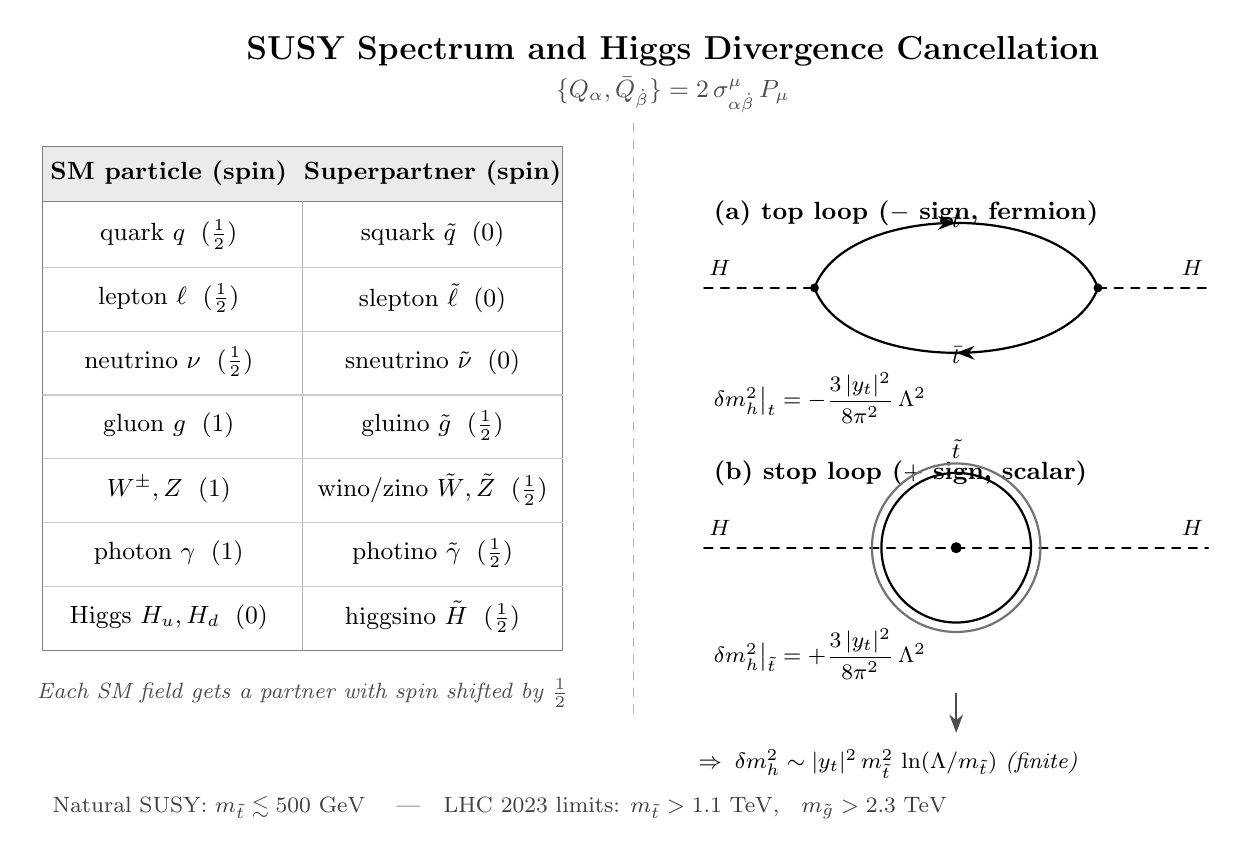
\begin{tikzpicture}[>=Stealth, line cap=round, line join=round]

% =============================================================
% Title
% =============================================================
\node[font=\large\bfseries] at (8.0,7.6) {SUSY Spectrum and Higgs Divergence Cancellation};
\node[font=\small,text=black!70] at (8.0,7.05)
  {$\{Q_\alpha,\bar{Q}_{\dot\beta}\} = 2\,\sigma^\mu_{\alpha\dot\beta}\,P_\mu$};

% =============================================================
% LEFT: SM <-> Superpartner table
% =============================================================
\begin{scope}[shift={(0,0)}]

% header band
\fill[black!8] (0,5.7) rectangle (6.6,6.4);
\draw[black!50] (0,5.7) rectangle (6.6,6.4);
\node[font=\small\bfseries] at (1.6,6.05) {SM particle (spin)};
\node[font=\small\bfseries] at (4.95,6.05) {Superpartner (spin)};

% body
\draw[black!50] (0,0.0) rectangle (6.6,5.7);
\draw[black!30] (3.3,0.0) -- (3.3,5.7);

% rows (7 rows, each 0.81 high)
\foreach \y in {0.81,1.62,2.43,3.24,4.05,4.86} {
  \draw[black!20] (0,\y) -- (6.6,\y);
}

% Row labels (top to bottom)
% Row 1: y=4.86..5.70  -- quark
\node[font=\small] at (1.6,5.28) {quark $q$ \;($\tfrac{1}{2}$)};
\node[font=\small] at (4.95,5.28) {squark $\tilde{q}$ \;(0)};
% Row 2: 4.05..4.86 -- lepton
\node[font=\small] at (1.6,4.47) {lepton $\ell$ \;($\tfrac{1}{2}$)};
\node[font=\small] at (4.95,4.47) {slepton $\tilde{\ell}$ \;(0)};
% Row 3: 3.24..4.05 -- neutrino
\node[font=\small] at (1.6,3.66) {neutrino $\nu$ \;($\tfrac{1}{2}$)};
\node[font=\small] at (4.95,3.66) {sneutrino $\tilde{\nu}$ \;(0)};
% Row 4: 2.43..3.24 -- gluon
\node[font=\small] at (1.6,2.85) {gluon $g$ \;(1)};
\node[font=\small] at (4.95,2.85) {gluino $\tilde{g}$ \;($\tfrac{1}{2}$)};
% Row 5: 1.62..2.43 -- W,Z
\node[font=\small] at (1.6,2.04) {$W^\pm,Z$ \;(1)};
\node[font=\small] at (4.95,2.04) {wino/zino $\tilde{W},\tilde{Z}$ \;($\tfrac{1}{2}$)};
% Row 6: 0.81..1.62 -- photon
\node[font=\small] at (1.6,1.23) {photon $\gamma$ \;(1)};
\node[font=\small] at (4.95,1.23) {photino $\tilde{\gamma}$ \;($\tfrac{1}{2}$)};
% Row 7: 0.0..0.81 -- Higgs
\node[font=\small] at (1.6,0.42) {Higgs $H_u,H_d$ \;(0)};
\node[font=\small] at (4.95,0.42) {higgsino $\tilde{H}$ \;($\tfrac{1}{2}$)};

% Caption under table
\node[font=\footnotesize\itshape, text=black!70] at (3.3,-0.55)
  {Each SM field gets a partner with spin shifted by $\tfrac{1}{2}$};

\end{scope}

% =============================================================
% Vertical separator
% =============================================================
\draw[black!30, dashed] (7.5,-0.8) -- (7.5,6.7);

% =============================================================
% RIGHT: Two Higgs self-energy diagrams
% =============================================================
\begin{scope}[shift={(8.4,0)}]

% ---- Top (top-quark) loop -----------------------------------
\node[font=\small\bfseries, anchor=west] at (0.0,5.55) {(a) top loop  ($-$ sign, fermion)};

% Higgs incoming/outgoing dashed lines
\draw[dashed, thick] (0.0,4.6) -- (1.4,4.6);
\draw[dashed, thick] (5.0,4.6) -- (6.4,4.6);
\node[font=\footnotesize] at (0.2,4.85) {$H$};
\node[font=\footnotesize] at (6.2,4.85) {$H$};

% Vertices
\fill (1.4,4.6) circle (1.6pt);
\fill (5.0,4.6) circle (1.6pt);

% Top loop (closed circle) with arrow direction
\draw[thick,
      decoration={markings, mark=at position 0.5 with {\arrow{Stealth}}},
      postaction=decorate]
  (1.4,4.6) .. controls (1.8,5.7) and (4.6,5.7) .. (5.0,4.6);
\draw[thick,
      decoration={markings, mark=at position 0.5 with {\arrow{Stealth}}},
      postaction=decorate]
  (5.0,4.6) .. controls (4.6,3.5) and (1.8,3.5) .. (1.4,4.6);

\node[font=\footnotesize] at (3.2,5.45) {$t$};
\node[font=\footnotesize] at (3.2,3.75) {$\bar{t}$};

% Result label for top
\node[font=\footnotesize, anchor=west] at (0.0,3.2)
  {$\delta m_h^2\big|_{t} = -\dfrac{3\,|y_t|^2}{8\pi^2}\,\Lambda^2$};

% ---- Stop (scalar) loop -------------------------------------
\node[font=\small\bfseries, anchor=west] at (0.0,2.25) {(b) stop loop  ($+$ sign, scalar)};

% Higgs incoming/outgoing dashed lines (single vertex tadpole)
\draw[dashed, thick] (0.0,1.3) -- (3.2,1.3);
\draw[dashed, thick] (3.2,1.3) -- (6.4,1.3);
\node[font=\footnotesize] at (0.2,1.55) {$H$};
\node[font=\footnotesize] at (6.2,1.55) {$H$};

% quartic vertex (4-point)
\fill (3.2,1.3) circle (2pt);

% Stop scalar loop (no arrow), drawn as a closed dashed-double curve
\draw[thick] (3.2,1.3) circle (0.95);
\draw[thick, black!55] (3.2,1.3) circle (1.07);

\node[font=\footnotesize] at (3.2,2.55) {$\tilde{t}$};

% Result label for stop
\node[font=\footnotesize, anchor=west] at (0.0,-0.05)
  {$\delta m_h^2\big|_{\tilde{t}} = +\dfrac{3\,|y_t|^2}{8\pi^2}\,\Lambda^2$};

% Sum / cancellation arrow
\draw[->, thick, black!70] (3.2,-0.55) -- (3.2,-1.05);

\node[font=\footnotesize, anchor=west] at (-0.2,-1.45)
  {$\Rightarrow\;\delta m_h^2 \sim |y_t|^2\,m_{\tilde{t}}^2\,\ln(\Lambda/m_{\tilde{t}})$ \textit{(finite)}};

\end{scope}

% =============================================================
% Footer notes
% =============================================================
\node[font=\footnotesize, text=black!75, anchor=west] at (0.0,-2.0)
  {Natural SUSY: $m_{\tilde{t}} \lesssim 500$ GeV \quad|\quad LHC 2023 limits: $m_{\tilde{t}} > 1.1$ TeV, \; $m_{\tilde{g}} > 2.3$ TeV};

\end{tikzpicture}
\end{document}
